\mcchap{La visualizzazione dati}{cap:breveStoria}
% spaziatura tra paragrafi
\setlength{\parskip}{1em}

\section{Cos'è la visualizzazione dati }
La rappresentazione grafica dei dati o in inglese \emph{data visualization} è l’attività di comunicazione realizzata tramite la proiezione di dati in una forma grafica strutturata.

\section{Breve storia}

Con la tecnologia moderna, la visualizzazione di dati non è mai stata così semplice.
Con pochi click si può trasformare un enorme tabella di dati grezzi in un diagramma accattivante e semplice da interpretare. Rappresentare i dati sotto forma di grafici, fornisce una via molto rapida per creare comprensione e far capire il proprio punto di vista.
Molte tecniche di visualizzazione dati che usiamo oggi furono inventate durante la prima rivoluzione industriale.
Quello che può sembrare semplice e ovvio oggi, come un grafico a linea o a barre,  sarebbe stato strano e sconosciuto a qualcuno 200 anni fa.

%\subsection{William Playfair}

Tra i primi pionieri della visualizzazione dati ci fu William Playfair, che tradusse dati in grafici nel 18esimo secolo. 

William Playfair, nella sua carriera tortuosa, oggi impensabile, si dedicò: allo spionaggio, all’ingegneria, alla redazione, alla contabilità, all’invenzione, alla lavorazione dei metalli e molto altro. La sua eredità eredità duratura risiede nel campo della statistica, con i grafici che ha progettato che costituiscono il nucleo della visualizzazione dei dati di oggi.

Ai tempi di Playfair, i dati venivano presentati in tabelle asettiche di non facile interpretazione con poca attenzione per la loro interpretazione. Se volevi capire qualcosa, non c’erano scorciatoie intuitive, dove solo dopo un laborioso lavoro di esaminare attentamente i numeri, ricordare, copiare e confrontare i dati.

%\subsection{William Playfair}

Nel 1765, arrivò il diagramma temporale di Joseph Priestley, che mostrava le vite sovrapposte di vari statisti e filosofi classici. 
Invece di elencare semplicemente nomi, anni di nascita e anni di morte, Priestley li tracciò su una linea temporale, rendendo immediatamente visibile quali personaggi storici fossero contemporanei.

\begin{figure}[htp]
    \centering
    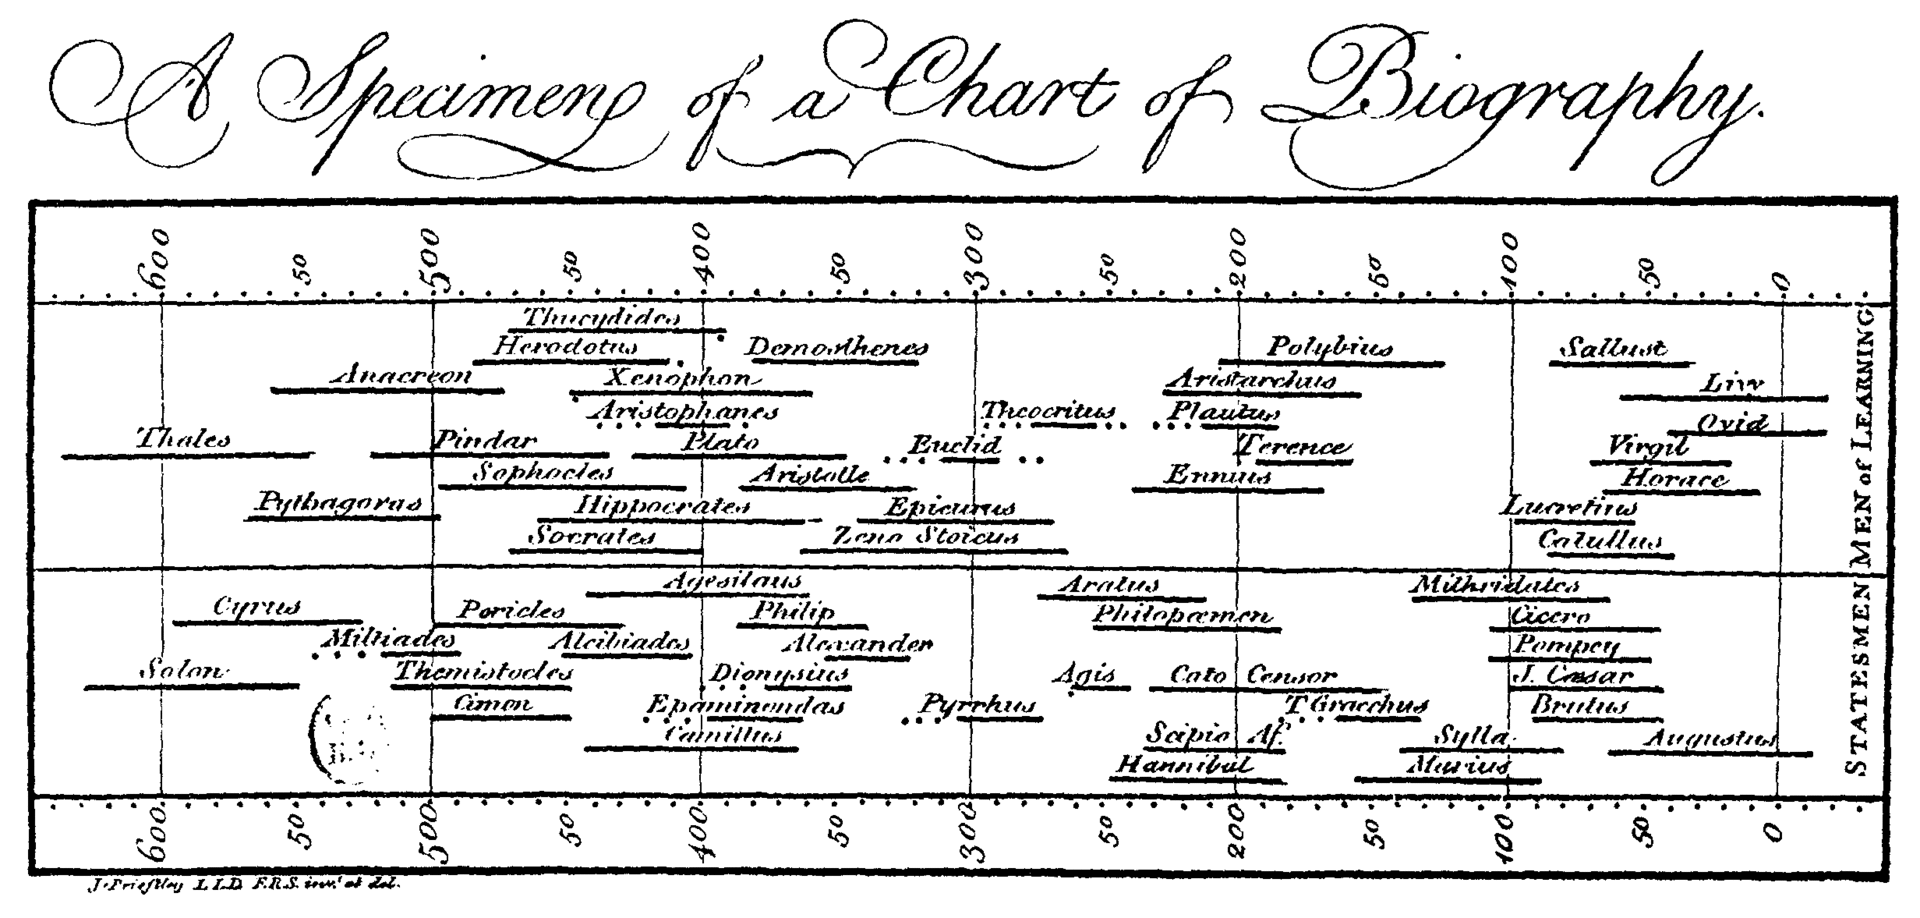
\includegraphics[width=10cm]{PriestleyChart}
    \caption{Joseph Priestley — Grafico sequenza temporale}
    \label{fig:PriestleyChart}
\end{figure}

Queste sequenze temporali si sono rivelate un successo e hanno ispirato direttamente l'invenzione del grafico a barre di Playfair, che apparve per la prima volta nel suo Atlante commerciale e politico.

\begin{figure}[htp]
    \centering
    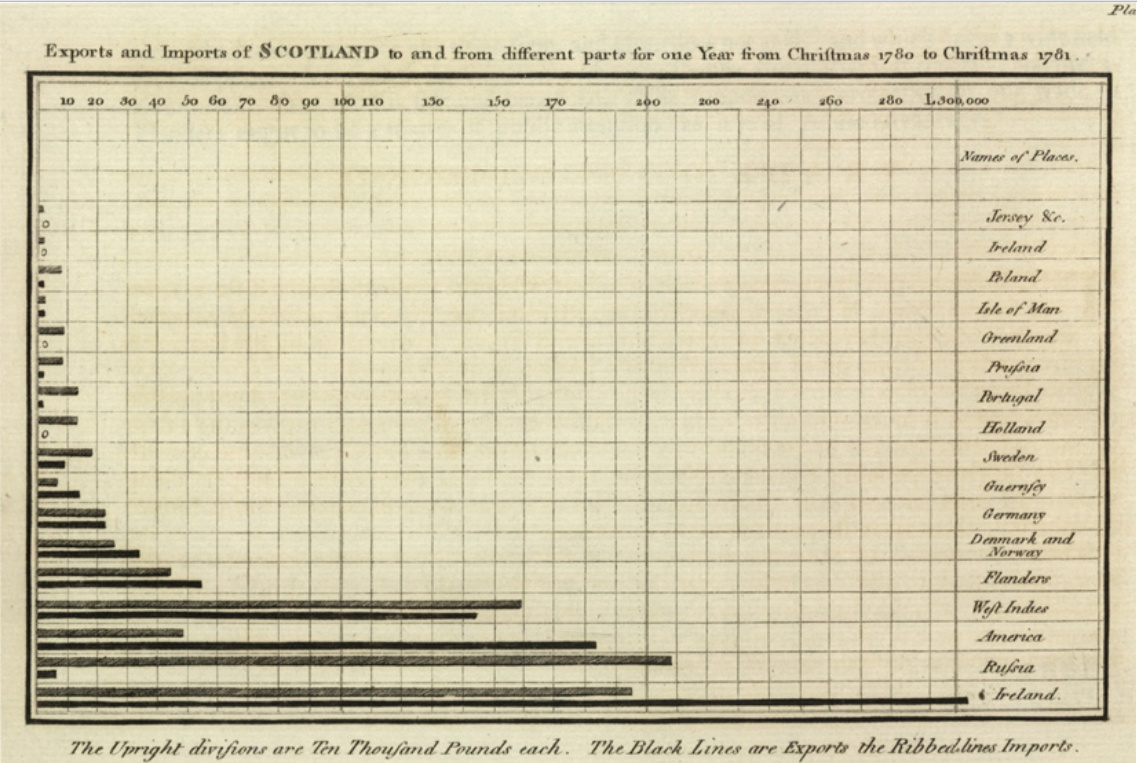
\includegraphics[width=9cm]{Playfair_chart}
    \caption{William Playfair — Atlante Politico e Commerciale}
    \label{fig:playfair_chart}
\end{figure}

Quindici anni dopo, Playfair era tornato con con il grafico a torta a volte controverso e varie combinazioni creative. È sorprendente pensare che, più di duecento anni dopo, le idee di un uomo costituiscano ancora la maggior parte delle opzioni grafiche in un software di visualizzazione dei dati all'avanguardia.

\begin{figure}[htp]
    \centering
    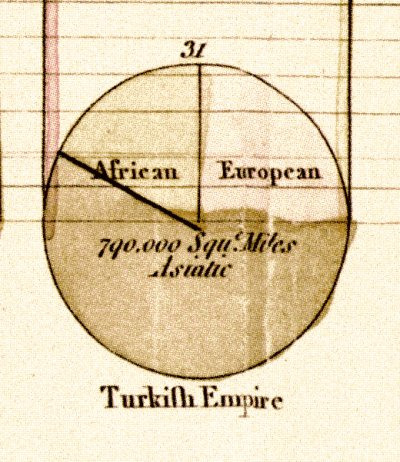
\includegraphics[width=6cm]{playfair_piechart}
    \caption{William Playfair — Grafico a torta}
    \label{fig:playfair_piechart}
\end{figure}




